% !TEX encoding = UTF-8
% !TEX spellcheck = en_US

\documentclass[10pt]{beamer}
\usepackage[utf8]{inputenc}
\usepackage[T1]{fontenc}
\usepackage{lmodern}

\usepackage{amsmath}
\usepackage{amsfonts}
\usepackage{amssymb}

\usepackage[style=authoryear,backend=bibtex]{biblatex}
\addbibresource{bibliography.bib}

\setbeamertemplate{itemize item}[square]
\setbeamertemplate{itemize subitem}[circle]

% Math symbols
\DeclareMathOperator{\Cat}{Cat}
\DeclareMathOperator{\Norm}{\mathcal N}
\DeclareMathOperator{\Id}{\mathbf I}

\newcommand{\vect}[1]{\boldsymbol{#1}} % make bold vector names

\begin{document}
\author{Giovanni Papini}
\title{Adversarial Autoencoders (AAE)}
\subtitle{Adattato da \cite{makhzani2015adversarial}}
%\logo{}
\institute{Universit\'a degli Studi di Firenze}
\date{12 febbraio 2019}
\subject{autoencoders, neural network, AI}
%\setbeamercovered{transparent}
%\setbeamertemplate{navigation symbols}{}

\begin{frame}[plain]
\maketitle
\end{frame}

\begin{frame}{Abstract}
\begin{itemize}
  \item Probabilistic autoencoder
  \item Use of the GAN framework
  \item Removing ``holes'' in the latent space
  \item Many applications:
  \begin{itemize}
    \item semi-supervised learning
    \item disentanglement of style and content of images
    \item unsupervised clustering
    \item dimensionality reduction
    \item data visualization
  \end{itemize}
\end{itemize}
\end{frame}

\begin{frame}{Context}
\begin{itemize}
  \item Scalable generative models to capture rich distributions
  \item Graphical models such as RBMs , DBNs, DBMs are based on MCMC algorithms for doing inference
  % via via sempre più imprecisi a causa dell'incapacità di mixing veloce tra le mode delle catene
  \item VAE, GAN, GMMN are trained via direct back-propagation
  \item The AAE is trained with dual objectives:
  % AE classico non regolarizzato ottiene una codifica troppo arbitraria e poco compatta
  \begin{itemize}
    \item minimizing the reconstruction error (classic AE)
    \item adversarial criterion that matches the aggregated posterior distribution of the latent representation to an arbitrary prior
  \end{itemize}
\end{itemize}
\end{frame}

\begin{frame}{The AAE architecture}
\begin{figure}
  \centering
  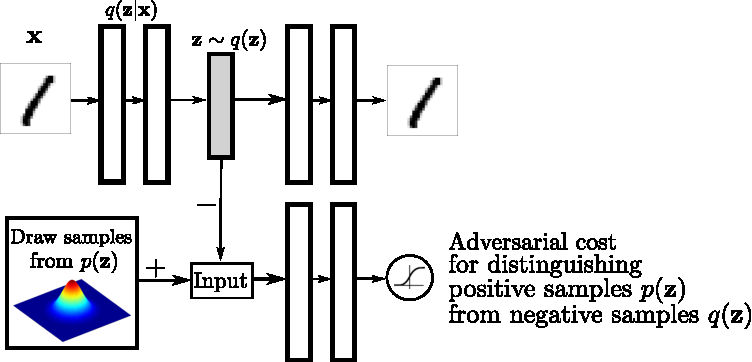
\includegraphics[width=0.8\linewidth]{../images/aae-architecture-01.png}
\end{figure}
\[ p(\vect z) = \int_{\Omega_x} q(\vect z | \vect x) p_d(\vect x) \text d \vect x \]
\end{frame}

\begin{frame}{Relationship with VAEs}
\begin{figure}
  \centering
  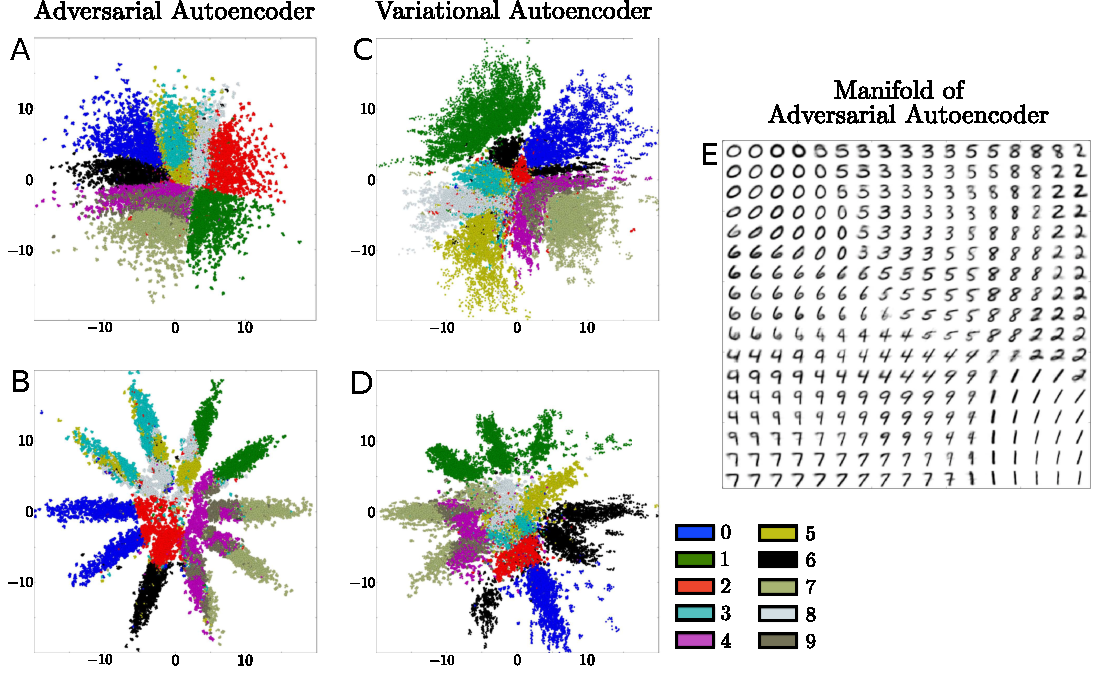
\includegraphics[width=0.8\linewidth]{../images/aae-embedding-01.png}
\end{figure}
\end{frame}

\begin{frame}{Relationship with GANs and GMMNs}
\centering
\begin{tabular}{c c}
  \textbf{GAN} & \textbf{AAE} \\ \hline
  \parbox{0.45\linewidth}{\begin{itemize} 
      \item imposes the data distribution to the output of a neural network 
    \end{itemize}} & 
  \parbox{0.45\linewidth}{\begin{itemize}
      \item relies on the autoencoder to capture the data distribution
      \item shapes a much lower dimensional space into a much simpler distribution
    \end{itemize}} \\
  \textbf{GMMN} & \textbf{AAE} \\ \hline
  \parbox{0.45\linewidth}{\begin{itemize}
      \item first trains a dropout autoencoder then fits a distribution in the code-space of the pretrained network
  \end{itemize}} &
  \parbox{0.45\linewidth}{\begin{itemize}
      \item uses adversarial training as a regularizer that shapes the code that shapes the code distribution while training the autoencoder from scratch
  \end{itemize}}
\end{tabular}
\end{frame}

\begin{frame}{Likelihood analysis}
\begin{itemize}
  \item Benchmarks on: MNIST, \href{../images/tfd.gif}{\underline{Toronto Face Dataset}} (TFD)
  \item Not direct likelihood measure, but lower bound approximation (KDE using Gaussian Parzen window)
\end{itemize}
\begin{figure}
  \centering
  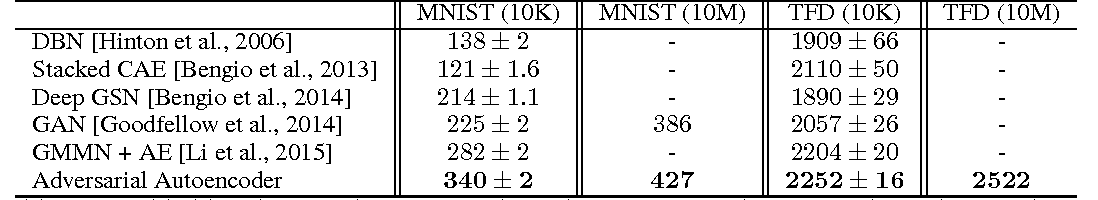
\includegraphics[width=\linewidth]{../images/performance-table-01.png}
\end{figure}
\end{frame}

\begin{frame}{Semi-supervised approach}{Architecture}
\begin{itemize}
  \item Incorporate one-hot vector in the latent representation
  \begin{figure}
    \centering
    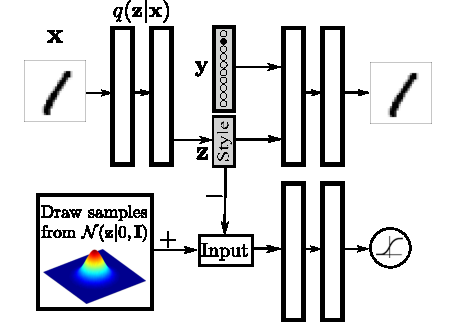
\includegraphics[width=0.6\linewidth]{../images/aae-architecture-02.png}
  \end{figure}
  \item The AAE disentangles \textit{style} features from \textit{content/semantic} features
  \item Experiments on MNIST and \href{../images/svhn.gif}{\underline{Street View House Number}} dataset (SVHN)
\end{itemize}
\end{frame}

\begin{frame}{Semi-supervised classification}{Architecture}
\begin{tabular}{cl}
  \begin{tabular}{c}
    \hspace{-0.5cm}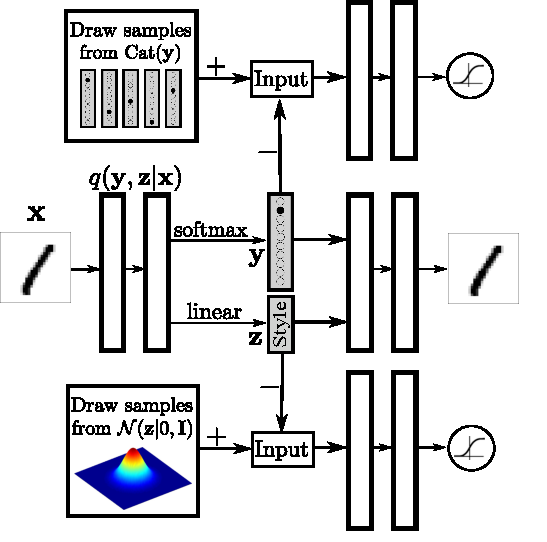
\includegraphics[width=0.45\linewidth]{../images/aae-architecture-03.png}
  \end{tabular} &
  \begin{tabular}{l}
    \hspace{-1cm}\parbox{0.6\linewidth}{% change the width as appropriate
      \begin{itemize}
        \item Improve classification performance using both labeled and unlabeled data
        \item Assume the latent space is a mixed Categorical and Gaussian distribution
        \[ p(\vect y) = \Cat(\vect y) \quad p(\vect z) = \Norm(\vect z; 0, \Id) \]
        \item For each distribution a different adversarial network regularizes the latent representation
    \end{itemize}}
  \end{tabular}
\end{tabular}
\end{frame}

\begin{frame}{Semi-supervised classification}{Training}
3-phase training:
\begin{enumerate}
  \item \textit{reconstruction} — the AE updates the encoder $ q(\vect z, \vect y | \vect x) $ to minimize the reconstruction error
  \item \textit{regularization} — each adversarial network
  \begin{itemize}
    \item first updates the discriminative network to distinguish true samples from the generated samples
    \item then update the encoder to confuse the discriminative networks
  \end{itemize}
  \item \textit{semi-supervised classification} — the AE updates $ q(\vect z, \vect y | \vect x) $ to minimize the cross-entropy cost on a labeled minibatch
\end{enumerate}
\end{frame}

\begin{frame}{Semi-supervised classification}{Results}
\begin{figure}
  \centering
  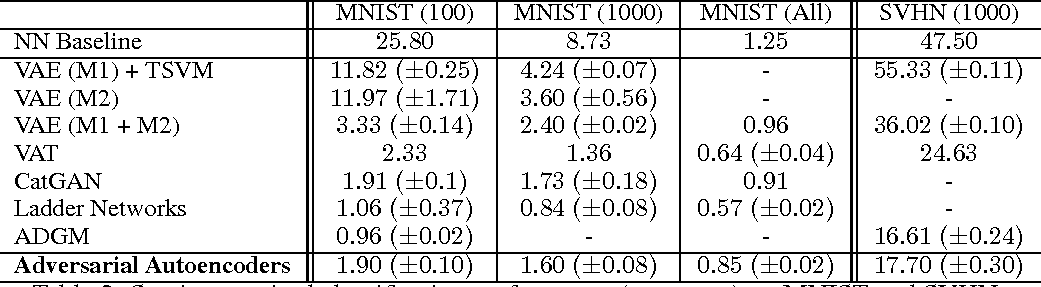
\includegraphics[width=\linewidth]{../images/performance-table-02.png}
\end{figure}
% AAE models are trained end-to-end while VAE models have to be trained one layer a time
\end{frame}

\begin{frame}{Unsupervised clustering}
\begin{itemize}
  \item 
\end{itemize}
\end{frame}

\begin{frame}{Dimensionality reduction}{Architecture}
\begin{figure}
  \centering
  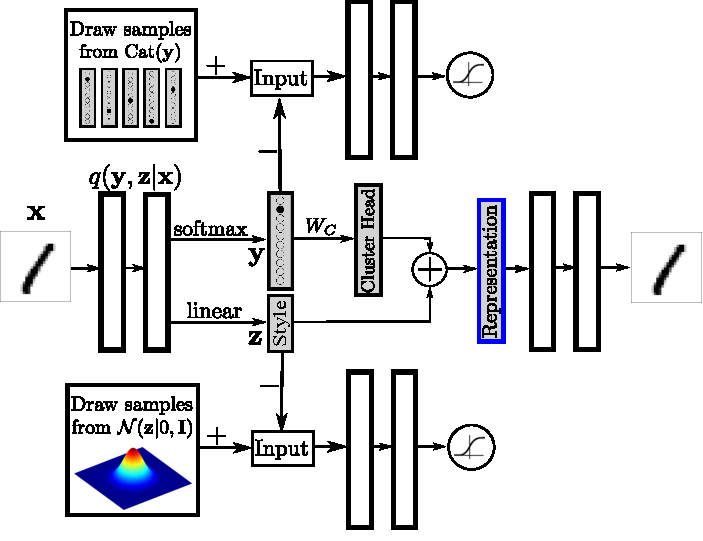
\includegraphics[width=0.8\linewidth]{../images/aae-architecture-04.png}
\end{figure}
\end{frame}

\begin{frame}{Conclusions}
\end{frame}

\begin{frame}{References}
\nocite{bengio2013better}
\nocite{bengio2014deep}
\nocite{goodfellow2014generative}
\nocite{kingma2013auto}
\printbibliography
\end{frame}

\end{document}